\begin{savequote}[75mm]
Nothing in Biology Makes Sense Except in the Light of Evolution
\qauthor{Theodosius Dobzhansky}
\end{savequote}

\chapter{Introduction}
\label{introduction}
\begin{flushleft}
\setlength{\parindent}{7ex}
\section{Disclosure}
Parts of this introduction, especially the section on Wnt signaling, have been adapted from own publications, including \textit{Wnt signaling in cancer} \cite{Zhan2017}

\section{The Colon and Colorectal Cancer}

Colorectal cancer is the third most common cancer worldwide and is associated with a Western lifestyle \cite{BrayGlobalCancerStatistics}. Similar to other solid tumors, colorectal adenocarcinoma progression is classified into four stages by the UICC (Union for International Cancer Control). These range from a \textit{carcinoma-in-situ}, a malignant patch of cells that has not yet breached the basal lamina of the intestinal mucosa (stage 0), to metastatic disease (stage 4).\par

Besides its clinical relevance, the colon is an attractive model organ for stem cell biology and translational research, given the accessibility of tissue samples through preventative colonoscopy as well as the ability to generate in-vitro organoid models from primary samples.

\subsection{The Colon Stem Cell Niche}

In order to understand the underlying principles of colorectal cancer development, or any cancer in general, it is advisable to turn to the stem cell biology governing the tissue's anatomy and function first \cite{CleversCancerStemCell}. The colon stem cell niche, or crypt, is the source of all epithelial cells lining the colon. Similar to the small intestine, Lgr5+ instestinal stemcells are located at the bottom of the crypt and continuously renew the epithelium by proliferating and, through displacement, pushing newly formed cells towards the colon's lumen.\par

This architecture serves multiple purposes, including protection of stem cells and the control of cell fate decisions across the epithelium \cite{cleversIntestinalCryptPrototype2013a}. Multiple developmental pathways, especially Wnt signaling, Notch, BMP and ERK MAPK signaling, govern cell identity in the intestinal niche \cite{Gehart2019}. The concentration of signaling cues for most of these pathways are organized in gradients along the crypt-lumen axis. For example, the concentration of stem cell identity maintaining Wnt and EGF ligands, secreted by mesenchymal crypt cells and REG4+ deep secretory cells, decreases as cells are pushed outside of the crypt  \cite{Sasaki2016}. In contrast, the effect of BMP ligands, which promote cell differentiation, increases as the concentration of BMP inhibitors (such as Noggin) derived from basal mesenchymal cells decreases \cite{heBMPSignalingInhibits2004}. In summary, as a cell is pushed outside the crypt by a continuous stream of proliferating cells, developmental signaling cues vanish and subsequent gene expression changes lead to differentiation. Similarly, if enterocyte-progenitors are moved back into the crypt, the ambient signaling leads to a reprogramming towards an intestinal stem cell state \cite{tettehReplacementLostLgr5Positive2016a}. \par

Given the spacial confinement of proliferate signals, the crypt architecture also leads to a protection against malignant transformation. At the bottom of the crypt, a neutral competition of proliferating intestinal stem cells leads to the removal of damaged cells that show a reduced proliferation rate relative to population of surrounding stem cells \cite{snippertIntestinalCryptHomeostasis2010a}. Given this neutral competition and the dependence on external signals to proliferate, dysfunctional or transformed cells have a higher likelihood of being removed from the niche unless they acquire a set of molecular alterations that render them independent from niche signals and increase their proliferative rate. \par

As mentioned above, the key signaling pathways that maintain stem cell properties in the crypt are canonical Wnt signaling, while BMP signaling reduces stem-like properties and EGF dependent ERK MAPK signaling stimulates cell proliferation \cite{cleversIntestinalCryptPrototype2013a}. Given their control over cell state and crypt integrity, the majority of early driver mutations found in colorectal cancer, such as loss of APC (Wnt signaling), activation of \textbeta-catenin (Wnt signaling), activation of KRAS (ERK MAPK), BRAF (ERK MAPK) and loss of SMAD4 (TGFb/BMP signaling) are found in these exact signaling pathways \cite{fearonMolecularGeneticsColorectal2011}. Of these mutations, especially mutations of APC and KRAS are frequently observed early in colorectal cancer development and are highly correlated with eachother (50\% of APC mutant tumors harbor mutations of KRAS). \par

In summary, the architecture of the colon stem cell niche and the signaling pathways maintaining its integrity determine the cellular fitness landscape of colon epithelial cells and through it the most common somatic mutations that enable escape from these determinants towards malignant transformation.

\subsection{Signaling Pathways controlling the Colon Stem Cell Niche and Tumorigenesis}

A limited set of signaling pathways both control the cell state in the colon stem cell niche and are frequently altered during tumorigenesis. These pathways include (i) Wnt signaling, (ii) ERK MAPK signaling, and (iii) TGFb/BMP signaling \cite{gehartTalesCryptNew2019a}. In the following section the mechanism of Wnt signaling and ERK MAPK signaling are discussed in more detail, as these two pathways are altered by Apc loss and Kras activation, respectively.

\begin{figure}[h]
\centering
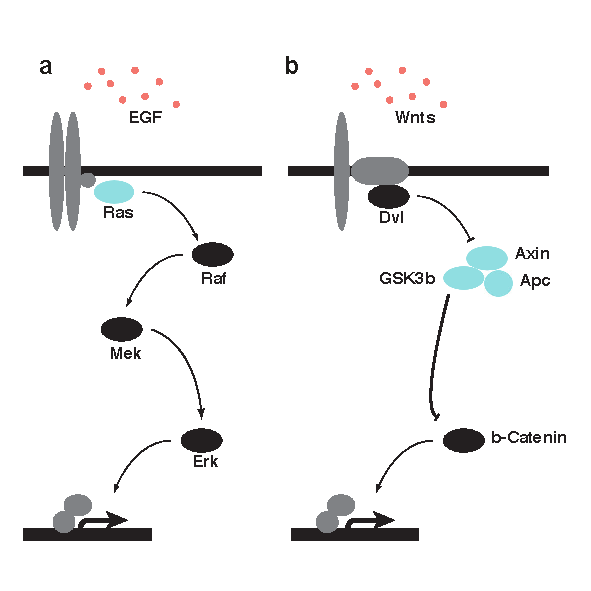
\includegraphics[width=0.7\textwidth,
                keepaspectratio]{figures/adenomaprofiling/pdf/fig_0_1.pdf}
\caption{\textbf{Simplified illustration of EGF dependent ERK-MAPK signaling and canonical Wnt signaling a} EGF dependent signaling cascade. Ras is highlighted in blue. \textbf{b} canonical Wnt signaling cascade. The destruction complex, including Apc, is highlighted in blue.}
\label{fig_180}
\end{figure}
\bigbreak

\subsubsection{Canonical Wnt Signaling}

In 1973, the wingless gene was discovered in a screen for visual phenotypes, affecting patterning processes in Drosophila melanogaster, the fruit fly \cite{Sharma1973WinglessMelanogaster.}. Subsequently, further genetic screens identified components of the Wnt family as key regulators during embryonic development and later, cancer initiation as well as stem cell maintanance  \cite{Nusslein-Volhard1980MutationsDrosophila}. \par 

In canonical Wnt signaling, absence of Wnt ligands leads to phosphorylation of \textbeta-catenin by the destruction complex, which contains the scaffold protein Axin, the large protein APC (Adenomatous polyposis coli) and the kinases GSK3\textbeta as well as casein kinase (CK1\textalpha) (reviewed in Zhan, Rindtorff et al.\cite{Zhan2017}). 
In this state, \textbeta-catenin is phosphorylated by GSK3\textbeta, ubiquitinated by \textbeta-TrCP and subsequently targeted for proteasomal degradation. 
In the absence of nuclear \textbeta-catenin, the trasncritpional repressive complex containing TCF/LEF and transducing-like enhancer protein (TLE/Groucho) recruits Histone deacetylases to repress target genes. \par 

The canonical pathway is activated upon binding of secreted Wnt ligands (for example, Wnt1 and Wnt 3a) to Fzd receptors and LRP co-receptors. 
Subsequently, LRP receptors are  phosphorylated by CK1\textalpha and GSK3\textbeta, which then recruits Dishevelled (Dvl) proteins to the plasma membrane where they polymerize and are activated \cite{Metcalfe2011}. Next, the Dvl polymers inactivate the destruction complex by sequestration in multivesicular bodies. This results in stabilization and accumulation of \textbeta-catenin which then translocates into the nucleus. There, \textbeta-catenin forms an active complex with LEF (lymphoid enhancer factor) and TCF (T-cell factor) proteins by displacing TLE/Groucho complexes which leads to the recruitment of histone modifying co-activators such as CBP/p300, BRG1, BCL9 and Pygo \cite{Lien2014WntSignaling}. \par 

Next to Wnt ligands, members of the R-spondin ligand family are positive effectors of Wnt signaling \cite{Kazanskaya2004, Glinka2011, Hao2012}. R-spondins bind to leucine-rich repeat containing G-protein-coupled receptors (Lgr) 4-6 \cite{Koo2012a}. In the absence of R-spondin, the two E3 ubiquitin ligases Znrf3 and Rnf43 target the Frizzled (Fzd) receptor for lysosomal degradation \cite{DeLau2011}. The interaction of ubiquitin ligases and receptrs is dependent on Dishevelled (Dsh).\cite{Jiang2015}. In the presence of external R-Spondins, binding of ligands to Lgr4-6 inhibits the activity of Znrf3/ Rnf43 and leads to the accumulation of Fzd receptors on the cell surface \cite{Hao2012, Koo2012a}. Being transcriptional targets of Wnt signaling themselves, Znrf3 and Rnf43 function as negative feedback regulators in Lgr5- positive cells \cite{DeLau2012}. \par 

The role of Wnt signaling during colorectal cancer development is well established \cite{Polakis2007}. While activating mutations of \textbeta-catenin do exist, loss of APC is the most frequent driver of Wnt signaling in colorectal cancer and can be found in about 80\% of colorectal cancer patients \cite{Fearon1989}. In line with its role as a tumor suppressor, truncating of APC using the CRISPR/Cas9 technology, leads to colorectal cancer development, which can be modeled ex vivo in human intestinal organoids \cite{Matano2015, Drost2015SequentialCells}. Furthermore, by using a mouse model allowing the reversible knockdown of Apc via shRNA, it was demonstrated that adenomas could regress to normal tissue once APC function is restored, underlining the importance of continuous Wnt signaling for tumor maintenance \cite{Dow2015}. \par
Although loss of APC in general is a driving event of colorectal cancer development and persistence, not every mutation of the APC gene leads to a similar phenotype. Studies of human colorectal cancer samples and tumors from mouse models revealed that different mutations of APC result in distinct levels of canonical Wnt pathway activity and, in addition, are associated with characteristic tumor locations within the large intestine \cite{Christie2013, Buchert2010}. \par

Besides APC, mutations in R-spondin and RNF43, regulators of Wnt receptor abundance at the cell surface level, 
were implicated as drivers of Wnt-dependent tumor growth \cite{Lau2014-zg}. Deleterious RNF43 mutations have been described in ~20\% of colorectal cancer cases and are mutually exclusive to APC mutations \cite{Giannakis2014-oq}. Also, amplified R-spondin3 fusion proteins have been described in 10\% of CRC cases \cite{R-spondin3}. RNF43 mutant cancers have a strong dependency on Wnt secretion, rendering them highly susceptible to Wnt secretion targeted therapy.

\subsubsection{ERK MAPK Signaling}

The extracellular-signal-regulated (ERK) mitogen-activated protein kinase family (MAPK) is one of three major MAPK families, together with the JNK (c-jun N-terminal kinase or stress-activated protein kinases) and MAPK14 group of protein kinases. These signaling cascades play a major role in (I) integrating external proliferative signals, (II) reacting to stress or ambient cytokines and (III) protecting cells from apoptosis, respectively \cite{Oncol2005}. 

In the colon crypt, the ERK MAPK signaling cascade and its members Ras-Raf-MEK and ERK are key regulators of cell proliferation. Blockade of EGF, a canonical ligand of the signaling cascade's upstream receptor EGFR, leads to a cell cycle arrest of proliferating Lgr5+ cells while not affecting their cellular state \cite{basakInducedQuiescenceLgr52017a}. As a result of the state preservation, cells can re-enter proliferation as soon as ERK MAPK signaling is restored.

In colorectal cancer, the Ras kinase members are mutated in about 36\% of cases \cite{Oncol2005}. According to the Vogelstein model of colorectal cancer initiation \cite{Fearon1989}, activating mutations of KRAS takes place early during cancer development, more specifically, after loss of APC.
Next to KRAS, BRAF mutations can also be found in around 10\% of colorectal cancers \cite{Oncol2005}. Of note, mutations of KRAS and BRAF occur mostly in a mutually exclusive pattern with BRAF mutations, which are enriched in Microsatellite instable colorectal cancers \cite{Oncol2005, Sahin2013}. 


\subsection{Colorectal Cancer Emergence and Therapy}

Cancer in general, and colorectal cancer in particular, is a disease marked by the accumulation of genetic events in somatic cells, which over time lead to uncontrolled growth and spread beyond the tissue of origin. Genetic characterization efforts have identified recurring somatic genetic events in colorectal cancer that appear during its progression. Both sequencing and functional genomics experiments have helped distinguish a subset of genetic events, so-called functional events or drivers, that cause a profound shift in cell state and lead towards cancer development. 

According to the adenoma-carcinoma sequence model, the majority of all colorectal adenocarcinomas arise from previously formed adenomas, benign neoplasms of the intestinal epithelium \cite{Cho1992}. As a consequence, one of the most effective medical interventions today to reduce death from colorectal cancer is the preventative removal of visible adenomas during lower endoscopy, such as colonoscopy \cite{Nishihara2013Long-TermEndoscopy}.\par

On a molecular level, colorectal adenocarcinoma can be organized into tumors arising through (I) a chromosomal instability or (II) a DNA-mismatch repair deficiency associated route \cite{Markowitz2009} (Figure \ref{colon_cancer_progression}). These two forms of tumor development have been associated with characteristic clinical, pathological, and molecular findings. For example, tumors of the DNA-mismatch repair phenotype are more frequently located in the right colon, have a higher proportion of microsatellite instability, frequent BRAF mutations and a higher immune-cell infiltration \cite{Markowitz2009}. In contrast, tumors of the common chromosomal instability (CIN) phenotype are mostly microsatellite stable and have frequent APC and KRAS mutations. \par 

The cascade of genetic events leading to the more frequent chromosomal instability associated form of colorectal cancer is known as the Vogelstein sequence \cite{Cho1992}. It starts with the loss of the tumor suppressor APC in the intestinal epithelium. Loss of APC, which leads to adenoma formation, is followed by the activation of KRAS, PIK3CA, loss of SMAD4 and TP53. Other forms of the disease, especially microsatellite-instable forms of colorectal cancer also harbor mutations of APC but show a higher prevalence of BRAF mutations instead of KRAS mutations \cite{Guinney2015TheCancer.}. \par 

The treatment of colorectal adenocarcinoma depends on disease stage. While surgical removal of the tumor is at the center of the treatment strategy, neoadjuvant and adjuvant chemotherapy are part of the recommended therapy from UICC stage 2 and 4 on, respectively. Today, for metastatic colorectal cancer the first line treatment includes combination chemotherapy (FOLFOX or FOLFIRI) paired with Cetuximab (anti-EGFR) for KRAS wildtype disease, combination chemotherapy with Bevacizumab (anti-VEGFR) for KRAS mutant disease or triple chemotherapy (FOLFOXIRI) in combination with Bevacizumab for BRAF mutant disease \cite{Cutsem}. Additional lines of therapy include different combinations of the aforementioned agents with the exception of Regorafenib and Triflouridin/Tipiracil as preferred third line agents for non-KRAS wildtype disease \cite{Cutsem}. Consequentially, the only genetic tests currently recommended during therapy are the determination of KRAS and BRAF status \cite{Cutsem}. Other genetic tests or targeted inhibitors have so far not found their way into clinical practice to date.\par

\section{Colon Organoids and Colorectal Cancer Organoids}

Organoids are three-dimensional cell culture models from primary adult tissue. Intestinal organoids develop from Lgr5+ adult stem cells and were first isolated from the small intestine of mice \cite{Sato2011}. Subsequently, following the initial publication, further organoid models across tissue-types and species have been developed. These include organoids from intact and cancerous human large intestine \cite{Sato2011}, pancreas \cite{Sachs2017}, mammary epithelium \cite{Zhang2016EstablishingCells, Sachs2017AHeterogeneity} and the hepatobiliary system \cite{Huch2013NIHAccess, Broutier2016CultureManipulation.}. The number of tissues that can be modeled through organoids has been continuously increasing since the first publication of this methodology. \par

Culturing organoids from primary cells requires the addition of specific tissue-dependent growth factors and the embedding of cells in 3D hydrogels \cite{Merker2016GastrointestinalOut}. In the case of colon organoids, the necessary growth factors are inspired by signaling cues available in the intestinal stem cell niche (discussed above): Wnt and R-spondin ligands to activate and maintain canonical Wnt signaling; EGF ligands to stimulate ERK MAPK signaling, and Noggin ligands to inhibit the differentiating effects of the BMP signaling cascade \cite{Sato2013}. When combined with inhibitors of TGF\textbeta and p38 mediated signaling, these growth factors enable organoid formation and continous proliferatation ex-vivo. In line with the niche-focused model of colon cancer formation outlined previously, patient derived colorectal cancer organoids proliferate in simpler conditions that correspond to their genetic state (i.e. APC mutant colon organoids grow in conditions lacking Wnt and R-spondin ligands) \cite{Fujii2016-de}. Not only the high isolation efficiency of up to 80\%, but also the high genetic and transcriptomic correlation with their tissue of origin have made organoids increasingly popular translational research model \cite{pauliPersonalizedVitroVivo2017a}. Both the high isolation efficiency, and the molecular representation of the tissue of origin are likely a result of the culture conditions which are mirroring the tissue-specific stem cell environment. These conditions reduce biases and evolutionary bottlenecks on the tissue's cells during the transfer into an in-vitro environment. \par

\subsection{Diagnostic use of Colorectal Cancer Organoids}

Given the benefits of the methodology, patient derived organoids are being trialed as predictive models for personalised treatment recommendation in colorectal cancer care \cite{VanDeWetering2015, Vlachogiannis2018, ganeshRectalCancerOrganoid2019a, ooftPatientderivedOrganoidsCan2019a, yaoPatientDerivedOrganoidsPredict2020a}. In these assays, personalised organoid models are generated and then treated with a candidate drug in-vitro. While robust reports on the predictive validity of organoids for progression-free survival are still missing, current results for response rate models show considerable predictive validity for Irinotecan, FOLFIRI, and neoadjuvant radiation therapy. A pooled analyses of the previously published literature recently summarised the aggregate sensitivity and specificity for organoid based treatment response rate prediction at 0.81 and 0.74, respectively (conservative single-point AUROC estimate: 0.78) \cite{wensinkPatientderivedOrganoidsPredictive2021, zhangNoteROCAnalysis2005}. For reference, a retrospective study of clinical experts estimated the predictive validity of an emergency room EKG for occlusive myocardial infarction at a sensitivity and specificity of 0.79 and 0.80, respectively (multi-point AUROC estimate: 0.80) \cite{al-zaitiMachineLearningECG2023}. Despite the potential of patient derived organoids to guide clinical decision making, the method is not ready for use in a clinical context with a high biopys-to-evaluation dropout rate and tunraround time being the primary technical hurdles. A recent failed single-arm prospective clinical trial for organoid-based last-line treatment recommendations reported a treatment for 6 out of 61 included patients (>90 \% dropout rate and 10 week turnaround time, 23 lost during organoid establishment, 11 lost due to disease progression) \cite{ooftProspectiveExperimentalTreatment2021}. Further improvements of reagents, isolation procedures, and in-vitro protocols might lead to lower dropout rates and turnaround times to enable further investigation of organoid-based diagnostics for personalised colorectal cancer care. \par

\subsection{Drug Discovery using Colorectal Cancer Organoids}

Next to diagnostics, organoid have been evaluated as models in drug discovery. Patient derived organoids can be processed in high-throughput small molecule screens with conventional cell viability readouts \cite{VanDeWetering2015}. However, besides testing therapeutic candidates on late stage cancer models, organoids are amenable to efficient genetic engineering \cite{Matano2015-zw, Drost2017-fu}. This opens up the possibility of evaluating the effect of therapeutic candidates against precisely defined genetic disease states. For example, organoid models with engineered tumor forming genetic changes, open up searching for therapeutic candidates that show effects specific to a given genetic event. As I will demonstrate throughout this thesis -specifically in the context of multi-genic somatic disease such as colorectal cancer- organoids are promising models for therapeutic discovery programs against (1) early and (2) progressed stages of this disease.

\section{Image-based Profiling in Therapeutic Discovery} 

Profiling experiments are biological experiments in which high dimensional phenotype data are collected for biological models that are subjected to multiple treatments \cite{chandrasekaranImagebasedProfilingDrug2021}. Examples for such methods include Transcriptome Profiling Experiments (Perturb-Seq, L1000 Profiling) as well as Image-based Profiling Experiments. These data intensive experiments generate three-dimensional data tensors containing phenotype profiles (i.e. transcript count or morphological feature) for multiple treatments (i.e. small molecules) and experimental units (i.e. conventional adherent cell lines or organoids). At this point it is important to note that the presence of dense phenotype information for multiple treatments (= causal interventions) is what separates profiling experiments from observational studies, such as -for example- single-cell RNA-Sequencing of multiple clinical samples. Image-based profiling is a high-throughput microscopy-based experimental methodology to systematically measure phenotypes of in-vitro models. When combined with chemical or genetic perturbations, image-based profiling experiments are a powerful approach to gain systematic insights into biological processes during therapeutic discovery projects. 

\subsection{Distinguishing Screening Experiments and Profiling Experiments in Therapeutic Discovery}

During Therapeutic Discovery, profiling experiments in general and image-based profiling experiments in particular have been adopted during the early stages of the discovery process: (1) the target identification phase, (2) hit identification phase, and (3) hit to lead transition phase \cite{chandrasekaranImagebasedProfilingDrug2021}. A hallmark of profiling experiments are coarse-grained and uncertainty-aware assumptions about the biological mechanism that is investigated and, as a result, an emphasis on the unbiased collection of phenotype information as well as the use of complex biological models with high clinical predictive validity. In practice a profiling experiment collects more information than needed to test a coarse-grained mechanistic hypothesis and can as a result also serve as a starting point for further mechanism discovery. 

To further illustrate the statement above, let's contrast profiling experiments against alternative and previously more common screening experiments. The first general steps in the design process of biological experiments are:

(1) definition of the experimental units, here the biological models that are studied (units u)
(2) definition of the treatments with which to perturb the models (treatments t)
(3) definition of the phenotypes that are measured by observing the treated biological models (phenotypes p)

Common, mechanistic, experimental designs are based on strong prior assumptions about the biological mechanism of interest. For example, in a Cancer Therapeutic Discovery project, candidates within a small molecule set might be hypothesised to exert a selective cytotoxic effect on cancer cells by inhibiting a protein kinase through ATP-competitive binding to its active site. A well designed experiment might involve a kinase binding assay in which the dissociation constant (phenotype p) of the set's small molecules (treatment t) relative to the kinase's catalytic domain (unit u) can be estimated. Such experiments, referred to as screening experiments when run at large scale, are effective to test potential treatments against a well defined mechanistic hypothesis. 

In contrast, profiling-focused experiments are based on weaker prior assumptions about the biological mechanism of interest, and -as a result- often use more complex, valid experimental units and collect more, high-dimensional phenotypes. To stay with the example of the Cancer Therapeutic Discovery project above, the weaker prior assumptions might be that candidates within the small molecule set change the growth pattern of cancer cells so that they are more similar to healthy epithelial cells. Such a coarse-grained hypothesis does not include assumptions about the expected mechanism of action of such a desired small molecule. The resulting design might include adherent cell lines from different tissues as experimental units and a set of hundreds of unbiased morphological features that are collected through automated microscopy as phenotypes. Such profiling experiments are effective to both test potential treatments against a coarse-grained mechanistic hypothesis and to extend said hypothesis by providing observations for further mechanism discovery. 

To further refine the distinction between profiling and screening experiments, let's reconsider our previous profiling experiment. If the rest of the experimental design was kept similar, but the high dimensional phenotype data was replaced with a one-dimensional ATP-based cell viability assay, the resulting experiment would be considered a phenotypic screening experiment, and not a profiling experiment. In a phenotypic screen a complex experimental unit, such as a cell, is perturbed and a single robust aggregate phenotype, such as the cell viability is measured. While phenotypic screens can be useful to test treatment against one hypothesised mechanism, a mechanism discovery problem presents itself, often referred to as "target deconvolution dilemma" by practioners: The experiment does not enable further reasoning about the unit's complex inner workings and the potential mechanisms of action of observed treatments. Put differently, there are many biological mechanisms through which a treatment could have let to the observed phenotype. Profiling experiments, in contrast, observe more data than would be sufficient to test the simple underlying mechanistic hypothesis - often hundreds to thousands of features for a given treatment and unit. When combined with additional labels, these enriched phenotype profiles can help guide through the "target deconvolution dilemma" by, for example, grouping treatments according to proposed mechanisms of action.

\subsection{Learning meaningful representations for image-based profiling experiments}

Besodes follow-up discriminative experiments to refine the mechanism - as any other highthrougput experiment to identifiy observations that are created by treatments adversarial to the experimental design, This requires 
* machine learning augmented interpretation of the resulting data - cite paper which I advised

Representation Space is key 
what do we describe the phenotype with?


Support Set -> interpretability and robustness of the representation space
* untreated untis (incl. negative control)
* well annotated treatements (incl. positive control)

the larger the support set the better the guarantees above

Central piece is the representation
Often learnt on all available data 
Can be a challenge if we are in an actual discovery process - i.e. target annotation for small molecules are avaiable only for a subset of the tested treatments 
in RNAi - do not confuse with query and target treatements that are used in combinations. 
intro support set and query set in this vain - I propose the use of these terms, term is new, but the practice is not

common methods for representation have been 
feature selection
unsupervised
self-supervised


Labels for units and treatments
Interpretable phenotype features

Support Set and Query Set
profile + label (unit)
profile + label treatment

Interpretable representations

The integration of image and transcriptome data into ensemble approaches has shown promise to improve MOA determination for synthetic small molecules, natural products and identified bioactive metabolites21,117.

guilt ba association with genetic background or treatment - generalisable through a support set 

by feature processing 
by interpretable support set

Procure or Engineer Target model and reference model
Distinguish Target phenotype and Reference phenotype


general purpose -> higher iteration speed given reduced design changes





In the context of image-based profiling the phenotype that is observed is the morphology of the biological model visualised through a set of unbiased, general purpose staining techniques. The benefits of image-based 


Support set of observations
diseased vs health cells from patients
different geneticall modified cells 
cell that are untreated und treated with a compound that is supposed to be imitaded 

Query set of observations
Test small molecules, identify moelcules that have a desireable trait

Profiling experiments should be so interpretable that they can stand in place for a variety of specific assays. Potentially to the point where they can - together with computer expeirments, a single step between computation-based and clinical experimentation


Image-based assays have been used to screen large libraries of small molecules to identify potential drug candidates, to analyze a drug’s mode-of-action, or to classify drug-gene interactions by cell-morphology20–23. 

\subsection{Examples of image-based profiling experiments in Therpeutic Discovery}

Recursion - cavernous malformaiton
Carpenter - predict MoA from images
Bernd Fischer



\subsection{Current limitations of image-based profiling}

predictive validity - if we see an effect we would like it to be real
models 3D Models
complex diseases 
Per- forming large image-based profiling experiments of organoids has been, however, a biological, technical and computational challenge24–26. As a consequence, the morphological hetero- geneity of patient-derived cancer organoids between and within patient donors, their diverging behaviors upon pharmacological perturbation as well as the underlying mechanisms of cancer organoid morphology are not yet systematically understood.


if we see an effect we would like to have a hypothesis why it happenend -> guide further decision making; drugs with mechanism have a higher chance of being approved
meaningful representations - collecting interpretable phenotypes - multi-view data - representation
gene info is interpretable - but also here peopel identify programs
morphology is more challenging - features are often not interpretable - commonly done is a PCA or other transformation into compressed
factorisation
there are labels for units and treatments, there are not yet interpretable phenotype features - especially in image-based profiling (other modalities have semantic concepts, such as a gene)


cost and scale - most affordable profiling method
can be made for accessible for collaborative discovery if we reduce technical overhead. I.e. brightfield microscopy as a common trunk 
increase reliability for scientists at different locations








\section{Aims of Thesis}
Here we report a large scale image-based phenotyping study of patient-derived cancer organoids to understand underlying fac- tors governing organoid morphology. Colorectal cancer orga- noids from 11 patients were treated with more than 500 experimental and clinically used small molecules at different concentrations. We systematically mapped the morphological heterogeneity of patient-derived organoids and their response to compound perturbations from more than 3,700,000 confocal microscopy images. We found that the resulting landscape of organoid phenotypes was mainly driven by differences in orga- noid size, viability and cystic vs. solid organoid architecture. Using multi-omics factor analysis for integrating organoid mor- phology, size, gene expression, somatic mutations and drug activity, we identified biological programs underlying these phe- notypes and small molecules that modulate them.

Our contributions are

\subsection{Establishing Image-based Profiling Experiments for Organoids}

Patient derived organoids (PDOs) are physiological 3D tumor models that can be efficiently derived from cancer and normal tissues.1–3 Organoid isolation from human primary tumors and metastases1,4 has enabled the establishment of living biobanks.2,3,5–7 Notably, patient derived organoids have been shown to represent their origin’s molecular features and morphology,2–4,8 enabling functional experiments such as drug testing ex vivo.3,5,9–14 
Image-based profiling is a high-throughput microscopy-based methodology to systematically measure phenotypes of in vitro models. By learning a lower dimensional representation of biological images, biological states can be described, quantified and deciphered. When scaled and combined with chemical or genetic perturbations, this becomes a powerful approach to gain systematic insights into biological processes, making it a popular method in drug discovery and functional genomics research.15–17. Image-based assays have for instance been used to screen large libraries of small molecules to identify potential drug candidates, to analyze a drugs mode of action, or to classify drug-gene interactions by cell-morphology.18–21 Recently, image-based profiling of monogenic disease models has been particularly relevant for drug discovery. Here, primary cells from diseased tissue are profiled, perturbed and candidate drugs reversing the phenotype from a diseased to a healthy cell morphology are prioritized for drug development or used as diagnostics.22,23
Previously, high-throughput image-based profiling experiments have mostly been performed in a limited number of adherent cell lines and not been available to a growing number of disease models that require more sophisticated culture conditions, such as models from diverse cancers, rare genotypes or personalized disease models. Performing image-based profiling experiments of patient derived cancer organoids, a prime example for a complex 3D polygenic disease model, are, however, a technical and biological challenge. While image-based drug testing in organoids have been performed, the morphological heterogeneity of patient-derived cancer organoids between and within patient donors as well as their diverging behavior upon molecular perturbations are not yet systematically understood.24–26
Here we report on a large-scale image based phenotyping study of patient derived cancer organoids. We generated patient derived organoids from colorectal cancer patients and treated 11 organoid models with more than 500 experimental and clinically used compounds at different concentrations. We systematically mapped the morphological heterogeneity of patient derived organoids and their response to compound perturbations from more  than  3,700,000  confocal microscopy images. We identified a heterogeneous landscape of organoid phenotypes mainly driven by differences in organoid size, viability and cystic vs. solid organoid architecture. Using multi-omics factor analysis, we identified biological programs underlying these phenotypes and compounds that modulate them. For example, we linked cystic organoid architecture with a LGR5+ enriched, Wnt signaling dependent organoid state that could be induced via MEK inhibition and organoid size to an IGF-1R driven organoid state that was relatively insensitive to EGFR inhibition and could be induced via mTOR inhibition. A better understanding of organoid phenotypes and the ability to use multi-omics data to annotate organoid states and their plasticity have the potential to further accelerate image-based drug discovery for complex multigenic diseases.


\subsection{Identification of molecular factors of colorectal cancer organoid architecture and plasticity}

\subsection{Demonstrating Small Molecule Profiling in a multi-step, multi-view model of colon cancer initiation}
\end{flushleft}

% First, we isolated and characterized patient derived colorectal cancer organoids. Next, we performed high- throughput drug profiling of these organoids. Here, we observed a variety of recurring treatment-induced phenotypes. These were linked to specific cellular processes. Of note, the treatment response of organoids in-vitro matched the response of donating patients.

% Second, we isolated colon organoids from healthy mouse tissue. By using gene-editing, we generated models of colon adenoma - a precursor lesion of colorectal cancer. These models carried different combinations of mutations in the Apc and Kras gene. Both are frequent and co-occurring mutations in colorectal cancer (Schell et al. 2016). To better understand the mechanisms of tumor development, we performed a multi- omics characterization in these adenoma models. Moreover, we profiled genotype specific drug effects. Here we found a reorganization of organoid phenotype after loss of Apc, which masks the effects of an isolated Kras mutation. Loss of Apc leads to genotype specific drug-induced phenotypes and vulnerabilities. Oncogenic Kras buffers a subset of these vulnerabilities, offering a new perspective on the relationship of Apc and Kras during tumor development.